\documentclass[article]{jss}
\usepackage{thumbpdf,lmodern} 
\graphicspath{{Figures/}}

\usepackage{amsmath}

\author{Jing Hua Zhao\\University of Cambridge
 \And Jian'an Luan\\University of Cambridge
 \And Peter Congdon\\University of London}
\Plainauthor{Jing Hua Zhao, Jian'an Luan, Peter Congdon}

\title{Bayesian Linear Mixed Model with Polygenic Effects}
\Plaintitle{Bayesian Linear Mixed Model with Polygenic Effects}

\Abstract{We considered Bayesian estimation of polygenic effects, in
  particular heritability in relation to a class of linear mixed models
  implemented in \proglang{R} \citep{R}. Our approach is applicable to
  both family-based and population-based studies in human genetics
  with which a genetic relationship matrix can be derived either from
  family structure or genome-wide data. Using a simulated and a real
  data, we demonstrate our implementation of the models in the generic
  statistical software systems \pkg{JAGS} \citep{JAGS} and
  \proglang{Stan} \citep{StanJSS} as well as several \proglang{R}
  packages. In doing so, we have not only provided facilities in
  \proglang{R} linking standalone programs such as \pkg{GCTA}
  \citep{yang11} and other packages in \proglang{R} but also addressed
  some technical issues in the analysis. Our experience with a host of
  general and special software systems will facilitate investigation
  into more complex models for both human and nonhuman genetics.}

\Keywords{Bayesian linear mixed models, heritability, polygenic effects,
relationship matrix, family-based design, genomewide association study}
\Plainkeywords{Bayesian linear mixed models, heritability, polygenic 
effects, relationship matrix, family-based design, genomewide association 
study}

\Address{
  Jing Hua Zhao, Jian'an Luan\\
  MRC Epidemiology Unit\\
  University of Cambridge School of Clinical Medicine\\
  Box 285, Institute of Metabolic Science\\
  Cambridge Biomedical Campus\\
  Cambridge CB2 0QQ\\
  United Kingdom\\
  E-mail: \email{jinghua.zhao@mrc-epid.cam.ac.uk},\email{jinghuazhao@hotmail.com},  \\
   \ \ \ \ \ \ \ \email{jianan.luan@mrc-epid.cam.ac.uk}\\
  URL: \url{https://jinghuazhao.github.io/}, \url{http://www.mrc-epid.cam.ac.uk/people/}\\

  Peter Congdon\\
  School of Geography and Life Sciences Institute\\
  Queen Mary\\
  University of London\\
  Mile End Road\\
  London E1 4NS\\
  United Kingdom\\
  E-mail: \email{p.congdon@qmul.ac.uk}\\
  URL: \url{http://www.geog.qmul.ac.uk/staff/congdonp.html}
}

\begin{document}


\section{Introduction}

The genetic basis of quantitative phenotypes has been a long-standing
research problem associated with a large and growing literature, and
one of the earliest was by \cite{fisher18} on additive effects of
genetic variants (the polygenic effects). In human genetics it is
common to estimate heritability, the proportion of polygenic variance
to the total phenotypic variance, through twin and family studies. For
twin studies, polygenic effects are embedded into correlations between
monzygotic and dizygotic twin pairs using the assumption that
monozygotic twins share all the genetic materials but dizygotic twins
only half. For family studies, the polygenic component is coupled with
a relationship matrix in a mixed model with covariates as fixed
effects, e.g., \cite{morton74} and \cite{lange02}.  The models differ
from those usually seen in general statistics as the polygenic effects
are represented by a random variable that is correlated among all
relatives due to genes shared identity-by-descent. The estimation can
be inaccurate due especially to shared environment in both twin and
family studies.

More recently, a large quantity of single nucleotide polymorphisms (SNPs), 
single base-pair variants of DNA, available from population-based samples 
has offered renewed interest in the problem. This is because the data 
allows for a genomic relationship matrix (GRM) to be built as part of a 
genomewide association study (GWAS) for identification and 
characterization of the DNA variants and phenotype (our outcome of 
interest) association. \cite{yang10} showed that a GRM can be used in the 
mixed model very much in the same way as in models for families where the 
relationship matrix is built on familial relationships. Consequently, the
ubiquitous availability of DNA also makes the models appropriate for any
samples with typed DNA polymorphisms. The approach is 
applicable to a wide variety of traits including continuous, discrete and 
time-to-event outcomes \citep{zhao12}. The estimation of heritability 
($h^2$), the proportion of total additive genetic variance as a proportion 
of total phenotypic variance, is fundamentally important since it largely 
quantifies the scope of a GWAS in gene discoveries and characterizations.

Bayesian methods are attractive since generic software systems are
available to facilitate the model-building, and they also help to
address the issue concerning the uncertainty in parameter
estimation. Moreover, they give credible intervals with highest
probability density (HPD) as opposed to frequentist interval
estimates, often derived under simplifying assumptions. Markov chain
Monte Carlo (MCMC) serves as a practical tool for Bayesian inference
with a full characterization of the posterior distribution of the
variance components as well as heritability. For this reason, Bayesian
methods have been widely used in plant and animal science literature
for a broad range of traits, e.g., \cite{yi00, varona05}. These
applications and the software employed almost exclusively use family
structure, given that the inverse of the relationship matrix is easily
calculated, as was also the case with work on humans, e.g.,
\cite{burton05}. Exceptions regarding software include package
\pkg{BLR} \citep{perez10, deloscampos13} in \proglang{R} \citep{R}
which can accommodate GRM but the analysis often has to be stopped due
to a nonpositive definite GRM. It is not obvious how these issues can
be addressed.

In our own analysis, we have encountered various issues.  Our attempts
to tackle these problems have led to some useful results, which we
believe will facilitate similar analyses by other colleagues.  Via a
simulated data and a real data, we implemented the models using
\pkg{JAGS} \citep[just another Gibbs sampler;][]{JAGS},
\proglang{Stan} \citep[sampling through adaptive
neighborhoods;][]{stan, StanJSS} and in the case of a large sample
package \pkg{BLR}. We wrote utilities in \proglang{R} to read or write
a GRM as generated from software \pkg{GCTA} \citep{yang11} to be used
with these software packages, which contain functions to calculate
heritability and its standard error when polygenic and residual
variance/standard errors are given. We further adapted the
\proglang{R} package \pkg{MCMCglmm} \citep{hadfield10} to enable
comparison between family-based or genotype-based relationship
matrices. These functions are available from the \proglang{R} package
\pkg{gap} \citep{gap,zhao07} with further information. We also gave
expressions for perturbing the covariance matrix when GRM is considered
nonpositive definite. We believe our work will be of interest in human
genetics as well as animal and plant genetics. Below we will briefly
describe the polygenic model, a simulated data as a benchmark and
an application. We then
conclude with a summary, which includes generic discussions on
non-genetic effects, missing outcomes, efficient implementation,
frequentist and Bayesian estimates of heritability for the \pkg{GCTA}
documentation example.

\section{Statistical models}

We start with an outline of the linear mixed model, showing 
how total additive genetic effects can be framed with respect to a 
relationship matrix. We then consider specification of the Bayesian 
linear mixed model.

\subsection{Linear mixed model}

To motivate we consider a study of body mass index (BMI, body weight/height (kg/m$^2$)) 
in relation to sex (0 = Man, 1 = Woman) and age (in years). A linear model 
(LM) of BMI on sex and age is as follows,
%
\begin{align}
\mbox{BMI} & = b_0 + b_1\ \mbox{sex} + b_2\ \mbox{age} + e \label{lm},
\end{align}           
%
where $b_0$ is an intercept, $b_1$ and $b_2$ are the regression 
coefficients for sex and age, indicating a unit change in BMI attributable 
to being a woman than man and per-year increase in age, respectively. $e$ 
is a residual term indicating effects on BMI other than sex and age. As 
will soon become clear, there is a need to have extra terms which are 
random variables, leading to a linear mixed model (LMM). More generally, 
let $y$ be a continuous variable and our outcome of interest, $X$ 
covariates, $u$ random effects. A LMM has the following form,
%
\begin{align}
y & =  X\beta + Zu + e \label{lmm},
\end{align}
%
where

$y$ -- an $N\times 1$ vector of observations;

$X$ -- an $N\times p$ matrix of known covariates;

$\beta$ -- a $p\times 1$ vector of unknown regression coefficients;

$Z$ -- a known $N\times q$ matrix of variables;

$u$ -- a $q\times 1$ vector of unknown random effects;

$e$ -- an $N\times 1$ vector of (unobservable random) errors.

We assume that $u\sim N(0, D)$ and $e\sim N(0, E)$, so that $y \sim 
N(X\beta, V)$ with $V = E + ZDZ^\top$.

Statistical inference of this model, based on the frequentist
approach, can be done with maximum likelihood (ML) or restricted
maximum likelihood (REML) estimation. Procedures are widely available
\citep[see][for further details]{sorensen02}.

\subsection{Linear mixed model with polygenic effects}

We assume that our trait of interest, $y$, is a function of $m$ causal
variants each with effect $u_i$, $u_i \sim N(0,\sigma_u^2)$,
$i=1,\ldots,m$, treated as random effect, $\sigma_u^2$ a polygenic
variance. These variants are DNA polymorphisms at particular positions
across the genome. At locus $i$, we assume the two causal alleles are
$q$ and $Q$ with frequency $1-f_i$, $f_i$, and forms genotypes $qq$,
$qQ$ and $QQ$, respectively with additive effects 0, 1, and 2. The
genotypic effects are associated following a Binomial distribution,
$\text{Bin}(2,f_i)$, with mean $2f_i$ and variance $2(1-f_i)f_i$,
respectively, leading to normalized additive effects ($z_i$) being
$-2f_i/\sqrt{2(1-f_i)f_i}$, $(1-2f_i)/\sqrt{2(1-f_i)f_i}$ and
$(2-2f_i)/\sqrt{2(1-f_i)f_i}$. The simplest form of a polygenic model
uses a linear combination of effects from all causal variants, i.e.,
$g=\sum_{i=1}^mz_iu_i$ where $z_i$ can be seen as a function of the
frequency of allele with effect acting as a scaling factor such that
$\E(z_i)=0$ and $\VAR(z_i)=1$. In matrix notation $g=Zu$, we have
$g\sim N(0,\sigma_u^2ZZ^\top)$ and $\sigma_g^2=m\sigma_u^2$ is the
variance of total additive effects (``polygenic effects''). From this
$\VAR(y)=\sigma_u^2ZZ^\top+\sigma^2I=\sigma_g^2ZZ^\top/m+\sigma^2I=\sigma_g^2A+\sigma^2I$,
where $A=ZZ^\top/m$ amounts to a relationship matrix and is indeed called
a GRM at the causal loci, $\sigma^2$ is the residual variance, and $I$
an identity matrix. Heritability is defined as the proportion of
phenotypic variance explained by the polygenic effects, namely,
$h^2 = \sigma_g^2 / (\sigma_g^2 + \sigma^2)$.

The matrix $A$ can be represented with genomewide data containing a large 
number ($M$) of SNPs analogous to causal variants, i.e., $G=WW^\top/M$ 
where $w_{ij}=(x_{ij}-2p_i)/\sqrt{2(1-p_i)p_i}$, $j=1,2,3$ represents the 
genotypic effects of SNP $i$ and $p_i$ is the allele frequency, while 
$x_{ij}=0, 1, 2$ for SNP $i$ having alleles $a_1$, $a_2$, and genotypes $a_1a_1$, $a_1a_2$, $a_2a_2$, 
respectively. A series of refinements of the $G$ matrix has been suggested 
by \cite{yang10}. The \pkg{GCTA} software can generate a compressed (.grm.gz) 
or binary (.grm.bin) form of GRMs from genomewide SNPs and provide REML 
estimates for the polygenic model.

In summary, our model is similar to (\ref{lmm}) in that $D = \sigma_g^2G$
and $E = \sigma^2I$, where $G$ is a GRM, 
\begin{align}
y & =  X\beta + g + e.\label{pm} 
\end{align}
$\VAR(y) = \sigma_g^2G+\sigma^2I$ with $g$ being ``polygenic effects'' and
$G$ an $N\times N$ GRM.

For data on relatives, the additive genetic relationship matrix $A$
can also be derived from a given family structure which is twice the
kinship matrix \citep{lange02} whose entries represent probabilities
of genes shared identity-by-descent among pairs of relatives. The
matrix can be generated by a number of \proglang{R} packages such as
\pkg{kinship2} \citep{kinship2} which are available from the
Comprehensive \proglang{R} Archive Network (CRAN).

\subsection{Bayesian linear mixed model with polygenic effects}\label{blmm}
A Bayesian linear mixed model (BLMM) with polygenic effects follows the set-up above, 
whose sampling model is as follows,
\begin{align}
y|\beta, u, \sigma^2 &\sim  N(X\beta+Zu, \sigma^2I),\nonumber\\
\beta|\sigma_\beta^2&\sim  N(0,\sigma_\beta^2B), \nonumber\\
u|\sigma^2 &\sim N(0,\sigma^2A),
\label{blmmp}
\end{align}
where $B$ is a known, nonsingular matrix and $\sigma_\beta^2$ is a 
hyperparameter. Full specification of the model is furnished with 
appropriate distributions for the variance components, e.g., Section~6.3
of \cite{sorensen02}. For the polygenic model (\ref{pm}) in this paper,
we have the likelihood and assumed prior specifications as follows:
\begin{align}
 y & \sim   N(\mu, \sigma^2I) \cr
 \mu & =  X\beta + g \cr
 \beta_j & \sim  N(0, 1000^2),\quad j=1,\ldots,p \label{blmms}, \cr
 g & \sim  N(0,\sigma_g^2G) \cr
 \sigma_g^2 & \sim \text{InvGamma}(s_1, s_2) \cr
 \sigma^2 & \sim \text{InvGamma}(s_1, s_2)
\end{align}
where $s_1$ and $s_2$ are chosen to provide noninformative priors, and the
matrix $B$ is diagonal.
Other priors for the variance components such as uniform are possible, 
as in Section~\ref{npd} below, see also \cite{waldmann09} and \cite{gelman06}.

\subsection{Handling of the $G$ matrix}
Simulation of the polygenic effects in Section~\ref{blmm} involves the
multivariate Normal distribution, which could be very time-consuming
when $N$ gets large. A speedup can be achieved by obtaining the
precision matrix as input to software described below. More often, a
Cholesky decomposition can be applied. For $g\sim N(0,\sigma_g^2G)$,
Let $G=CC^\top$ and $z_i \sim N(0,1)$, $i=1,\ldots,N$, then
$g_i=\sigma_g C z_i\sim N(0,\sigma_g^2G)$.  As expression
(\ref{blmms}) is amenable to a few software environments for MCMC
sampling, these are exposed in Section~\ref{bayes} below.

\section{Benchmark}

Data from \cite{meyer89} as in \cite{tempelman04} is used as our
benchmark. The pedigrees for each of these 282 animals derive from an
additional 24 base population (Generation 0) animals that do not have
records of their own, nevertheless are of interest with respect to the
inference on their own additive genetic values. Furthermore, it is
presumed that these original 24 base animals are not related to each
other. Therefore, the row dimension of $u$ is $306$ $(282+24)$. To
facilitate discussions the data is made available in package \pkg{gap}
available from the Comprehensive \proglang{R} Archive Network (CRAN)
at \url{https://CRAN.R-project.org/package=gap}.

\subsection{Frequentist approach}

\cite{tempelman04} gave a variety of estimates using \pkg{SAS} 
\citep{SAS-STAT}. We are interested in the REML estimates which are 
available from package \pkg{regress} \citep{clifford06}.
%
\begin{Schunk}
\begin{Sinput}
R> set.seed(1234567)
R> meyer <- within(meyer, {
+    y[is.na(y)] <- rnorm(length(y[is.na(y)]), 
+      mean(y, na.rm = TRUE), sd(y, na.rm = TRUE))
+    g1 <- ifelse(generation == 1, 1, 0)
+    g2 <- ifelse(generation == 2, 1, 0)
+    id <- animal
+    animal <- ifelse(!is.na(animal), animal, 0)
+    dam <- ifelse(!is.na(dam), dam, 0)
+    sire <- ifelse(!is.na(sire), sire, 0)
+  })
R> G <- kin.morgan(meyer)$kin.matrix * 2
R> library("regress")
R> r <- regress(y ~ -1 + g1 + g2, ~ G, data = meyer)
R> r
\end{Sinput}
\begin{Soutput}
Likelihood kernel: K = g1+g2

Maximized log likelihood with kernel K is  -843.962 

Linear Coefficients:
    Estimate Std. Error
 g1  222.994      1.429
 g2  238.558      1.760

Variance Coefficients:
    Estimate Std. Error
 G    31.672     13.777
 In   72.419     10.182
\end{Soutput}
\begin{Sinput}
R> with(r, h2G(sigma, sigma.cov))
\end{Sinput}
\begin{Soutput}
Vp = 104.091 SE = 9.925092 
h2G = 0.3042677 SE = 0.1147779 
\end{Soutput}
\end{Schunk}
%
Note that we deliberately filled the missing data according to the 
observed (we will relax this later on), then employed the 
\verb/kin.morgan/ function to obtain the kinship matrix, which is in 
turn used by the \verb/regress/ function from package \pkg{regress}.
We have $h^2(\mathit{SE})=0.30$ $(0.11)$.

\subsection{Bayesian approach}\label{bayes}

We now turn to the Bayesian approach and begin with a generic
implementation based on the \proglang{BUGS} (Bayesian inference using
Gibbs sampling) specification. As most such implementations would
involve large samples, we moved away from \pkg{WinBUGS} \citep{lunn00}
and used \pkg{OpenBUGS} \citep{OpenBUGS} and \pkg{JAGS} under
Linux. Both allow for command line execution but as noted earlier
\citep{R2WinBUGS} data manipulation is required which can be greatly
facilitated with \pkg{OpenBUGS}, specifically using the \proglang{R}
package \pkg{R2OpenBUGS} \citep{R2WinBUGS}. We focused on \pkg{JAGS}
as it was better tuned under Linux with \pkg{LAPACK}
\citep{anderson99}, or \pkg{Intel MKL}, \citep{MKL} and the
\proglang{R} counterpart \pkg{R2jags} \citep{R2jags}. We use multiple
chains (e.g., 2 to 4), and Brooks-Gelman-Rubin (BGR) statistics,
provided in \pkg{JAGS} or \proglang{Stan}, to check
convergence. Initial parameter values are generally based on subject
matter knowledge and/or parameter estimates from classical estimation.

\subsubsection[JAGS]{\pkg{JAGS}}
First, we prepare the data in \proglang{R} and call \pkg{JAGS}
via \pkg{R2jags},
%
\begin{Schunk}
\begin{Sinput}
R> C <- chol(G)
R> N <- dim(meyer)[1]
R> data <- with(meyer,
+    list(N = N, y = y, g1 = g1, g2 = g2, u = rep(0, N), GI = solve(G)))
R> inits <- function() list(b1 = 0, b2 = 0, tau.p = 0.03, tau.r = 0.014)
R> parms <- c("b1", "b2", "p", "r", "h2")
\end{Sinput}
\end{Schunk}
%
We apply inverse gamma priors.
%
\begin{Schunk}
\begin{Sinput}
R> modelfile <- function() {
+    b1 ~ dnorm(0, 0.000001)
+    b2 ~ dnorm(0, 0.000001)
+    tau.p ~ dgamma(0.001, 0.001)
+    tau.r ~ dgamma(0.001, 0.001)
+    sigma.p <- 1 / sqrt(tau.p)
+    sigma.r <- 1 / sqrt(tau.r)
+    g[1:N] ~ dmnorm(u[], GI[, ] / p)
+    for (i in 1:N) {
+      y[i] ~ dnorm(b1 * g1[i] + b2 * g2[i] + g[i], tau.r)
+    }
+    p <- pow(sigma.p, 2)
+    r <- pow(sigma.r, 2)
+    h2 <- p / (p + r)
+  }
R> library("R2jags")
R> jagsfit <- jags(data, inits, parms, modelfile, n.chains = 2, 
+    n.burnin = 500, n.iter = 5000)
\end{Sinput}
\end{Schunk}
%
Like \pkg{OpenBUGS}, the Normal distribution in \pkg{JAGS} is specified 
with respect to the precision. The \verb/solve/ function returns the 
inverse so it is only calculated once. The results are very close to the REML 
estimates.
%
\begin{Schunk}
\begin{Soutput}
Inference for Bugs model at "/tmp/RtmpBDC/model69497abe523a.txt", fit using
 jags, 2 chains, each with 5000 iterations (first 500 discarded), n.thin = 4 
 n.sims = 2250 iterations saved
          mu.vect sd.vect     2.5%      25%      50%      75%    97.5%  Rhat
b1        222.922   1.470  220.115  221.900  222.900  223.901  225.852 1.001
b2        238.520   1.735  235.074  237.358  238.555  239.656  241.806 1.001
h2          0.300   0.080    0.155    0.240    0.297    0.354    0.464 1.002
p          31.810  10.188   15.497   24.306   30.809   37.979   55.090 1.001
r          73.335   8.316   57.824   67.558   73.265   78.609   89.974 1.005
deviance 2181.332  25.940 2125.879 2164.537 2183.027 2199.645 2229.083 1.002
         n.eff
b1        2200
b2        2200
h2         820
p         1700
r          370
deviance  1900

For each parameter, n.eff is a crude measure of effective sample size,
and Rhat is the potential scale reduction factor (at convergence, Rhat=1).

DIC info (using the rule, pD = var(deviance)/2)
pD = 336.4 and DIC = 2517.8
DIC is an estimate of expected predictive error (lower deviance is better).
\end{Soutput}
\end{Schunk}
%
The version with Cholesky decomposition is as follows, noting that the 
factored matrix needs to be transposed.
%
\begin{Schunk}
\begin{Sinput}
R> data <- with(meyer, list(N = N, y = y, g1 = g1, g2 = g2, C = t(C)))
R> inits <- function() list(b1 = 0, b2 = 0, sigma.p = 0.03, sigma.r = 0.014)
R> modelfile = function() {
+    b1 ~ dnorm(0, 0.001)
+    b2 ~ dnorm(0, 0.001)
+    sigma.p ~ dunif(0, 1000)
+    sigma.r ~ dunif(0, 1000)
+    p <- pow(sigma.p, 2)
+    r <- pow(sigma.r, 2)
+    tau <- pow(sigma.r, -2)
+    g[1:N] <- sigma.p * C[, ] %*% z[]
+    for (i in 1:N) { 
+      z[i] ~ dnorm(0, 1) 
+    }
+    for (i in 1:N) { 
+      y[i] ~ dnorm(b1 * g1[i] + b2 * g2[i] + g[i], tau) 
+    }
+    h2 <- p / (p + r)
+  }
R> jagsfit2 <- jags(data, inits, parms, modelfile, n.chains = 2, 
+    n.burnin = 500, n.iter = 5000)
\end{Sinput}
\end{Schunk}
%
where we also used uniform priors for the variance components. Tthe
results are similar.
%
\begin{Schunk}
\begin{Soutput}
Inference for Bugs model at "/tmp/RtmpBDC/model69493125f2e2.txt", fit using
 jags, 2 chains, each with 5000 iterations (first 500 discarded), n.thin = 4
 n.sims = 2250 iterations saved
          mu.vect sd.vect     2.5%      25%      50%      75%    97.5%  Rhat
b1        222.131   1.422  219.462  221.142  222.115  223.023  225.001 1.001
b2        237.450   1.749  234.014  236.310  237.479  238.592  240.985 1.004
h2          0.305   0.081    0.158    0.247    0.301    0.363    0.465 1.001
p          32.690  10.297   16.105   25.196   31.516   39.138   55.136 1.001
r          73.642   8.845   57.751   67.597   72.856   79.268   92.616 1.002
deviance 2181.013  26.007 2127.094 2164.740 2182.502 2198.604 2228.893 1.001
         n.eff
b1        2200
b2        2200
h2        2200
p         2200
r         1200
deviance  2200

For each parameter, n.eff is a crude measure of effective sample size,
and Rhat is the potential scale reduction factor (at convergence, Rhat=1).

DIC info (using the rule, pD = var(deviance)/2)
pD = 338.2 and DIC = 2519.2
DIC is an estimate of expected predictive error (lower deviance is better).
\end{Soutput}
\end{Schunk}
%
\subsubsection[Stan]{\proglang{Stan}}
We further experimented with \proglang{Stan}, which is appealing to us as it
implemented faster sampling algorithms \citep[p.~307]{gelman14}. We worked
on both the \proglang{R} interface, \pkg{rstan} \citep{rstan}, and the command
line version, \pkg{cmdstan} \citep{cmdstan}.
%
\begin{Schunk}
\begin{Sinput}
R> data <- with(meyer, list(N = N, y = y, g1 = g1, g2 = g2, G = G))
R> library("rstan")
R> meyer.stan <- "
+  data {
+    int N;
+    vector[N] y;
+    vector[N] g1;
+    vector[N] g2;
+    matrix[N, N] G;
+  }
+  transformed data {
+    matrix[N, N] C;
+    C = cholesky_decompose(G);
+  }
+  parameters {
+    vector[2] b;
+    vector[N] z;
+    real sigma_p2;
+    real sigma_r2;
+  }
+  transformed parameters {
+    real sigma_p;
+    real sigma_r;
+    vector[N] g;
+    sigma_p = sqrt(sigma_p2);
+    sigma_r = sqrt(sigma_r2);
+    g = sigma_p * C * z;
+  }
+  model {
+    b ~ normal(0, 1000);
+    sigma_p2 ~ inv_gamma(0.001, 0.001);
+    sigma_r2 ~ inv_gamma(0.001, 0.001);
+    z ~ normal(0, 1);
+    y ~ normal(b[1] * g1 + b[2] * g2 + g, sigma_r);
+  }
+  generated quantities {
+    real h2;
+    real p;
+    real r;
+    p = sigma_p2;
+    r = sigma_r2;
+    h2 = p / (p + r);
+  }
+  "
R> parms <- c("b", "p", "r", "h2")
R> f1 <- stan(model_code = meyer.stan, data = data, chains = 2, iter = 500, 
+    verbose = FALSE)
R> f2 <- stan(fit = f1, data = data, chains = 2, iter = 5000, pars = parms,
+    verbose = FALSE)
\end{Sinput}
\end{Schunk}
%
where results from the first \verb/stan/ call is used as input to the
second call. Note that the program is sectioned with \verb/data/
passed from \proglang{R} and the part which is in
\verb/transformed data/. These are followed by \verb/parameters/ and
\verb/transformed parameters/ before they are used in
\verb/model/. Our quantities of interest can further be obtained from
\verb/generated quantities/.

The results from \proglang{Stan} are shown below and in
Figure~\ref{meyer:stan},
%
\begin{Schunk}
\begin{Soutput}
Inference for Stan model: df0c4ce12df598b4fcdd553dfe7d2cee.
2 chains, each with iter=5000; warmup=2500; thin=1; 
post-warmup draws per chain=2500, total post-warmup draws=5000.
 
        mean se_mean     sd    2.5%     25%     50%     75%   97.5%
b[1] 223.002   0.034  1.486 220.196 222.000 222.931 223.991 226.104
b[2] 238.582   0.036  1.765 235.219 237.396 238.534 239.729 242.170
p     32.082   0.308 10.407  14.705  24.671  30.850  38.697  55.176
r     73.372   0.216  8.501  57.613  67.483  72.975  78.737  91.190
h2     0.301   0.003  0.082   0.149   0.245   0.297   0.356   0.470
     n_eff  Rhat
b[1]  1955 1.000
b[2]  2385 1.000
p     1144 1.001
r     1555 1.000
h2    1051 1.001

Samples were drawn using NUTS(diag_e) at Fri Mar 30 17:55:39 2018.
For each parameter, n_eff is a crude measure of effective sample size,
and Rhat is the potential scale reduction factor on split chains (at 
convergence, Rhat=1).

Potential scale reduction factors:

     Point est. Upper C.I.
b[1]          1       1.00
b[2]          1       1.00
p             1       1.01
r             1       1.00
h2            1       1.01
lp__          1       1.01

Multivariate psrf

1
\end{Soutput}
\end{Schunk}
%
where the BGR diagnostic statistics show convergence of the
parameters.  The overlapped density plots for the two chains are also
shown in Figure~\ref{meyer:stan}.
\begin{figure}[t!]
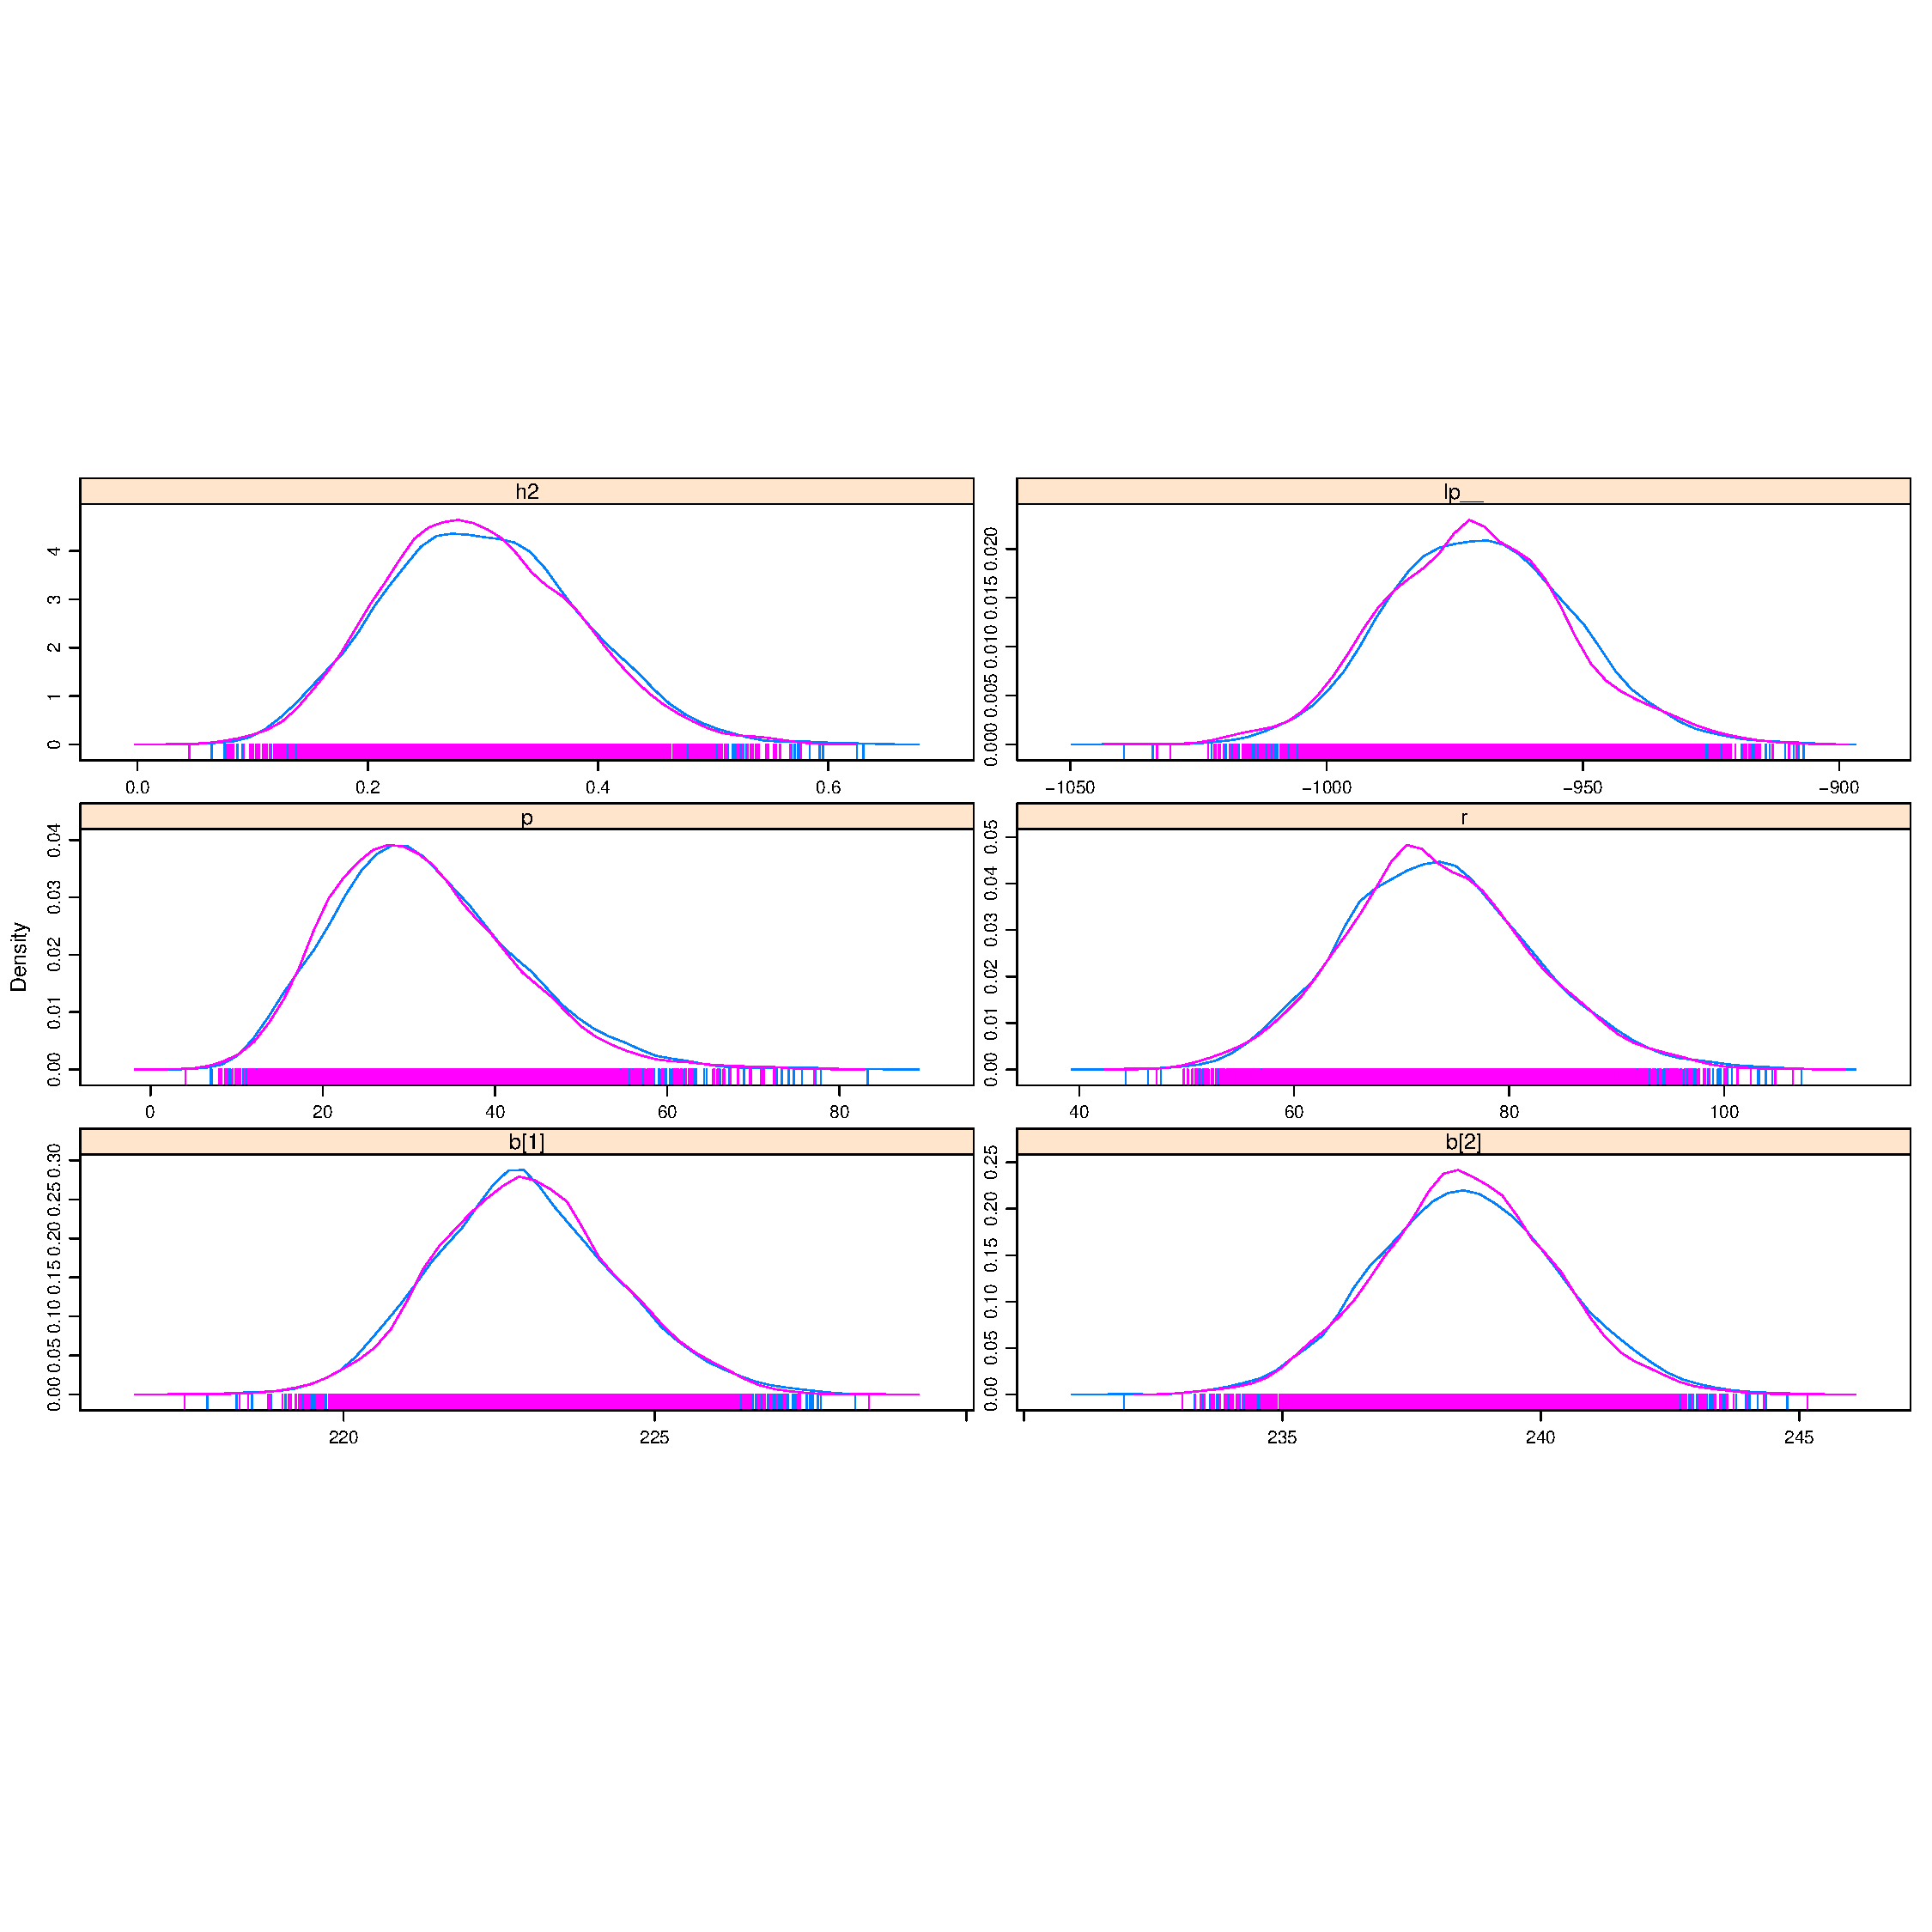
\includegraphics[width=\textwidth, trim = 0 260 0 260, clip]{jss2367-010}
\centering
\caption{Density plot for the Meyer data from \proglang{Stan}.}
\label{meyer:stan}
\end{figure}

Although both \pkg{OpenBUGS} and \pkg{JAGS} work as standalone programs, 
the counterpart in \proglang{Stan}, \pkg{cmdstan}, is much easier. We simply 
need to make a copy of the program above, say \texttt{meyer.stan}, to the 
\pkg{cmdstan} directory and issue ``\code{stanc}'' to generate the \proglang{C++} 
source or even ``\code{make meyer}'' to generate the executable, We first 
prepare for our data in \proglang{R} and then use functions 
\verb/bugs.data/ and \verb/bugs2jags/ to output an input file for \verb/meyer/,
%
\begin{Schunk}
\begin{Sinput}
R> library("R2OpenBUGS")
R> data <- with(meyer, list(N = N, y = y, g1 = g1, g2 = g2, G = G))
R> bugs.data(data, data.file = "meyer_bugs.txt")
\end{Sinput}
\begin{Soutput}
[1] "meyer_bugs.txt"
\end{Soutput}
\begin{Sinput}
R> library("coda")
R> bugs2jags("meyer_bugs.txt", "meyer_stan.txt")
\end{Sinput}
\end{Schunk}
%
and we can call
%
\begin{CodeChunk}
\begin{CodeInput}
$ ./meyer sample data file=meyer_stan.txt output file=meyer.csv
$ stansummary meyer.csv
\end{CodeInput}
\end{CodeChunk}
%
The data file (\code{meyer\_stan.txt}) is used by the executable to generate our 
output in \texttt{meyer.csv}, and the summary statistics are given by the 
\verb/print/ utility. Equally, \pkg{rstan} can also pick up results to 
allow for graphical facilities in \proglang{R}.

\section{Additional considerations}\label{additions}

\subsection{Parallel computation}\label{pc}
It is possible to take advantage of multicore facility in \proglang{R} for 
multiple chains via package \pkg{parallel} \citep{R}. 
This can be done as follows using the Meyer data.

\subsubsection[JAGS]{\pkg{JAGS}}
%
\begin{Schunk}
\begin{Sinput}
R> attach(meyer)
R> library("R2jags")
R> out <- jags.parallel(data, inits, parms, modelfile, n.chains = 4, 
+    n.burnin = 500, n.iter = 5000)
R> detach(meyer)
\end{Sinput}
\end{Schunk}
%
Note that the data needs to be attached.

\subsubsection[Stan]{\proglang{Stan}}
%
\begin{Schunk}
\begin{Sinput}
R> library("parallel")
R> parms <- c("b", "p", "r", "h2")
R> f1 <- stan(model_code = meyer.stan, data = data, chains = 4, iter = 500,
+    verbose = FALSE)
R> l <- mclapply(1:4, mc.cores = 4, function(i)
+    stan(fit = f1, seed = 12345, data = data, iter = 5000,
+      chains = 1, chain_id = i, refresh = -1))
R> f2 <- sflist2stanfit(l)
\end{Sinput}
\end{Schunk}
%
One can use the \verb/detectCores()/ function to obtain the number of cores
on the system and here four chains are run in parallel. Alternatively, a
call can be made with
%
\begin{Schunk}
\begin{Sinput}
R> options(mc.cores = parallel::detectCores() - 1)
\end{Sinput}
\end{Schunk}
%
\subsection[Nonpositive definite G matrix]{Nonpositive definite $G$ matrix}\label{npd}

We found it more likely to have a nonpositive definite $G$ matrix in
(\ref{blmmp}) and (\ref{blmms}) than a kinship matrix. In theory, we
can get around this with a perturbation ($\epsilon$) as described in
\citet[p.~174]{guo91}, namely to replace $G$ with
$\tilde G\equiv(G+\epsilon/\sigma_g^2I)$, so that
$\sigma_g^2\tilde G=\sigma_g^2G+\epsilon$ and
$\tilde\sigma^2=\sigma^2-\epsilon$ one only needs to amend $\sigma^2$
as $\tilde\sigma^2 + \epsilon$. The is according to the Gerschgorin
theorem \citep[Theorem 1.4]{varga04} as popularized by ridge
regression.
%
\begin{Schunk}
\begin{Sinput}
R> modelfile <- function() {
+    b1 ~ dnorm(0, 0.000001)
+    b2 ~ dnorm(0, 0.000001)
+    sigma.p ~ dunif(0, 1000)
+    sigma.r ~ dunif(0, 1000)
+    p <- pow(sigma.p, 2)
+    r <- pow(sigma.r, 2)
+    tau <- pow(sigma.r, -2)
+    g[1:N] ~ dmnorm(u[], inverse(p * G[, ] + eps * I[, ]))
+    for (i in 1:N) {
+      y[i] ~ dnorm(b1 * g1[i] + b2 * g2[i] + g[i], tau)
+    }
+    h2 <- p / (p + r)
+  }
\end{Sinput}
\end{Schunk}
%
This will be the same as before when $\epsilon=0$. While this is   
mathematically viable, it involves additional matrix inversion in
\pkg{JAGS} making our task even more formidable for MCMC convergence.
We used $(G+\epsilon I)$ in place of the relationship matrix and 
$\sigma^2+\epsilon\sigma_g^2$ as residual variance, which do not
involve direct simulation from the multivariate Normal distribution.

\section[Application: Familial vs. genomic heritabilities]{Application: Familial vs.~genomic heritabilities}\label{fgh}

The data used in this section was derived from a large family study which
mirrors work by \citep{klimentdis13}, to enable contrasting genetic relationship
from family structure and genome-wide data.

\newpage
\subsection{Frequentist approach}\label{fgh:freq}
Two relationship matrices based on family structure and genomic data
were generated by \proglang{R} and \pkg{GCTA}, respectively, to be used
by \pkg{GCTA} for REML estimation.

The genetic relationship matrix was built from pedigree structures
with package \pkg{kinship2} \citep{kinship2},
%
\begin{Schunk}
\begin{Sinput}
R> trios <- read.table("trios.dat", header = TRUE)
R> library("kinship2")
R> kmat <- with(trios, kinship(id, fid, mid))   
R> id <- trios[c("pid", "id")]
R> N <- dim(trios)[1]
R> M <- rep(N, N * (N + 1) / 2)
R> library("gap")
R> WriteGRM("PRM", id, M,  2 * kmat)
\end{Sinput}
\end{Schunk}
%
which was used by \pkg{GCTA} for REML estimates. Assuming that
phenotype information is stored in \code{p.dat}, \pkg{GCTA} can be called as follows,
%
\begin{CodeChunk}
\begin{CodeInput}
$ gcta64 --reml --grm-gz PRM --pheno p.dat --out PRM --thread-num 10
\end{CodeInput}
\end{CodeChunk}
%
The GRM as with REML estimates were obtained with \pkg{GCTA} as follows,
%
\begin{CodeChunk}
\begin{CodeInput}
$ gcta64 --reml --grm-gz GRM --pheno p.dat --out GRM --thread-num 10
\end{CodeInput}
\end{CodeChunk}
%
Note the calls to \pkg{GCTA} should be run under the Linux shell directly. 
The results are shown in Table~\ref{fgh_tab},
where $l_0$ and $l$ are the log-likelihoods with and without the polygenic
component, respectively. \pkg{GCTA} gave estimates of heritability which  
was remarkably similar, where $h^2(\mathit{SE})$ equals 0.46 (0.02) and 0.47
(0.03) with adjustment for sex and age, respectively for genome-based and
family-based estimates. One may rather use genomic structure as it is
associated with a greater likelihood.

\begin{table}[t!]
\centering\label{fgh_tab}
\begin{tabular}{rrrrr}
\hline
    &    \multicolumn{2}{c}{Genomic data} &    
\multicolumn{2}{c}{Family structure}\\ \cline{2-3} \cline{4-5}
    &    Variance     &          &  Variance    &     \\	
    &    components   &    SE    &  components  &     SE \\
\hline
$\sigma_g^2$ &   10.38  & 0.64 &  10.61   &  0.74\\
$\sigma^2$ &   12.33  & 0.50 &  12.01   &  0.63\\
$h^2=\sigma_g^2/(\sigma_g^2+\sigma^2)$  & 0.46 &    0.02  &  0.47&    0.03 \\
$l_0$        &   $-13479.85$  &      &       $-13572.17$  \\
$l$          &   $-13724.35$  &      &       $-13724.35$ \\
$\chi^2 = -2(l-l_0)$     &    489.00    &      & 304.36 \\
\hline
\end{tabular}
\caption{Estimates based on familial and genomic relationship matrices.}
\end{table}
\subsection{Bayesian approach}

Besides results from REML shown above, in a separation analysis on lung 
function from the same cohort, the two approaches yielded almost 
identical heritability estimates \citep{klimentdis13}. The marked 
difference in deviance prompted us to seek to characterize variability of 
heritability in a Bayesian framework.

For this ``large $N$'' ($N \gg 1,000$) problem, the implementation in
either \pkg{JAGS} or \proglang{Stan} became prohibitively slow, we
therefore resorted to specific implementations in packages
\pkg{MCMCglmm} and \pkg{BLR} that we were aware of. However, an
adaption of package \pkg{MCMCglmm} with GRM took about three days on
our Linux system with 300 burn-ins and 1,000 iterations and it is
infeasible to consider large number of iterations. With package
\pkg{BLR}, we encountered the issue of nonpositive definite GRM. While
adding a perturbation to the GRM it was not clear how our results will
be adjusted.  We also sought for the possibility of approximate
Bayesian methods through which \pkg{AnimalINLA} \citep{holand13} came
to our attention. It was derived from package \pkg{INLA} \citep[integrated
nested Laplace approximation;][]{rue14}. It was not obvious it can
handle GRM but we would like to explore.

First, we set up the data to be used,
%
\begin{Schunk}
\begin{Sinput}
R> pheno <- read.table("p.dat", col.names = c("pid", "id", "r"))
R> N <- nrow(pheno)
R> is.na(trios[trios == 0]) <- TRUE
R> f <- merge(pheno, trios[, -1], by = "id", all = TRUE)
R> p <- data.frame(f[with(f, order(pid, id)), ], u = seq_len(N),
+    e = seq_len(N))
R> rownames(p) <- seq_len(N)
\end{Sinput}
\end{Schunk}
%
\subsubsection[AnimalINLA]{\pkg{AnimalINLA}}

The \pkg{AnimalINLA} package was used first taking family structures
into account.

\subsubsection{Using family structure}
%
\begin{CodeChunk}
\begin{CodeInput}
R> library("AnimalINLA")
R> library("pedigree")
R> trios <- add.Inds(p[c("id", "fid", "mid")])
R> trios[is.na(trios)] <- 0
R> data <- merge(trios, p[c("id", "r")], by = "id", all.x = TRUE)
R> nr <- nrow(data)
R> p2 <- data.frame(data, u = 1:nr, e = 1:nr)
R> p2 <- within(p2,id <- as.integer(id))
R> xx <- compute.Ainverse(p2[c("id", "fid", "mid")])
R> fit <- animal.inla(response = "r", fixed = NULL, 
+    genetic = "id", Ainverse = xx, type.data = "gaussian",
+    data = p2, sigma.e = TRUE, dic = TRUE)
\end{CodeInput}
\end{CodeChunk}
%
where package \pkg{pedigree} \citep{coster13} is called to fill up nonexistent individuals.
The computation was done in minutes on our Linux with the default setup 
and the output is as follows,
%
\begin{CodeChunk}
\begin{CodeInput}
R> with(fit, summary.hyperparam)
\end{CodeInput}
\begin{CodeOutput}
                      mean         sd 0.025quant   0.5quant 0.975quant
Heritability     0.4638121 0.02627007  0.4107825  0.4644854  0.5139594
Variance for id 10.5297315 0.68491690  9.2106374 10.5260495 11.8806914
Variance for e  12.1992915 0.55650775 11.1555301 12.1825397 13.3272536
\end{CodeOutput}
\end{CodeChunk}
%
The \proglang{S}3 \code{plot} method for the returned
`\code{Animalinla}' object always sets \verb/xlim = c(0, 1)/ and
created plots on the console so we revised this.
%
\begin{CodeChunk}
\begin{CodeInput}
R> par(mfrow = c(3, 1))
R> plot(fit$sigma.u, type = "l", ylab = "Posterior",
+    xlab = expression(paste(sigma[u]^2)))
R> plot(fit$sigma.e, type = "l", ylab = "Posterior",
+    xlab = expression(paste(sigma^2)))
R> plot(fit$gaussian.h, type = "l", ylab = "Posterior",
+    xlab = expression(paste(h^2)), xlim = c(0, 1))
\end{CodeInput}
\end{CodeChunk}
%
The posterior distribution of $h^2$ is shown in Figure~\ref{fgh:animalinla}.

\begin{figure}[t!]
\centering
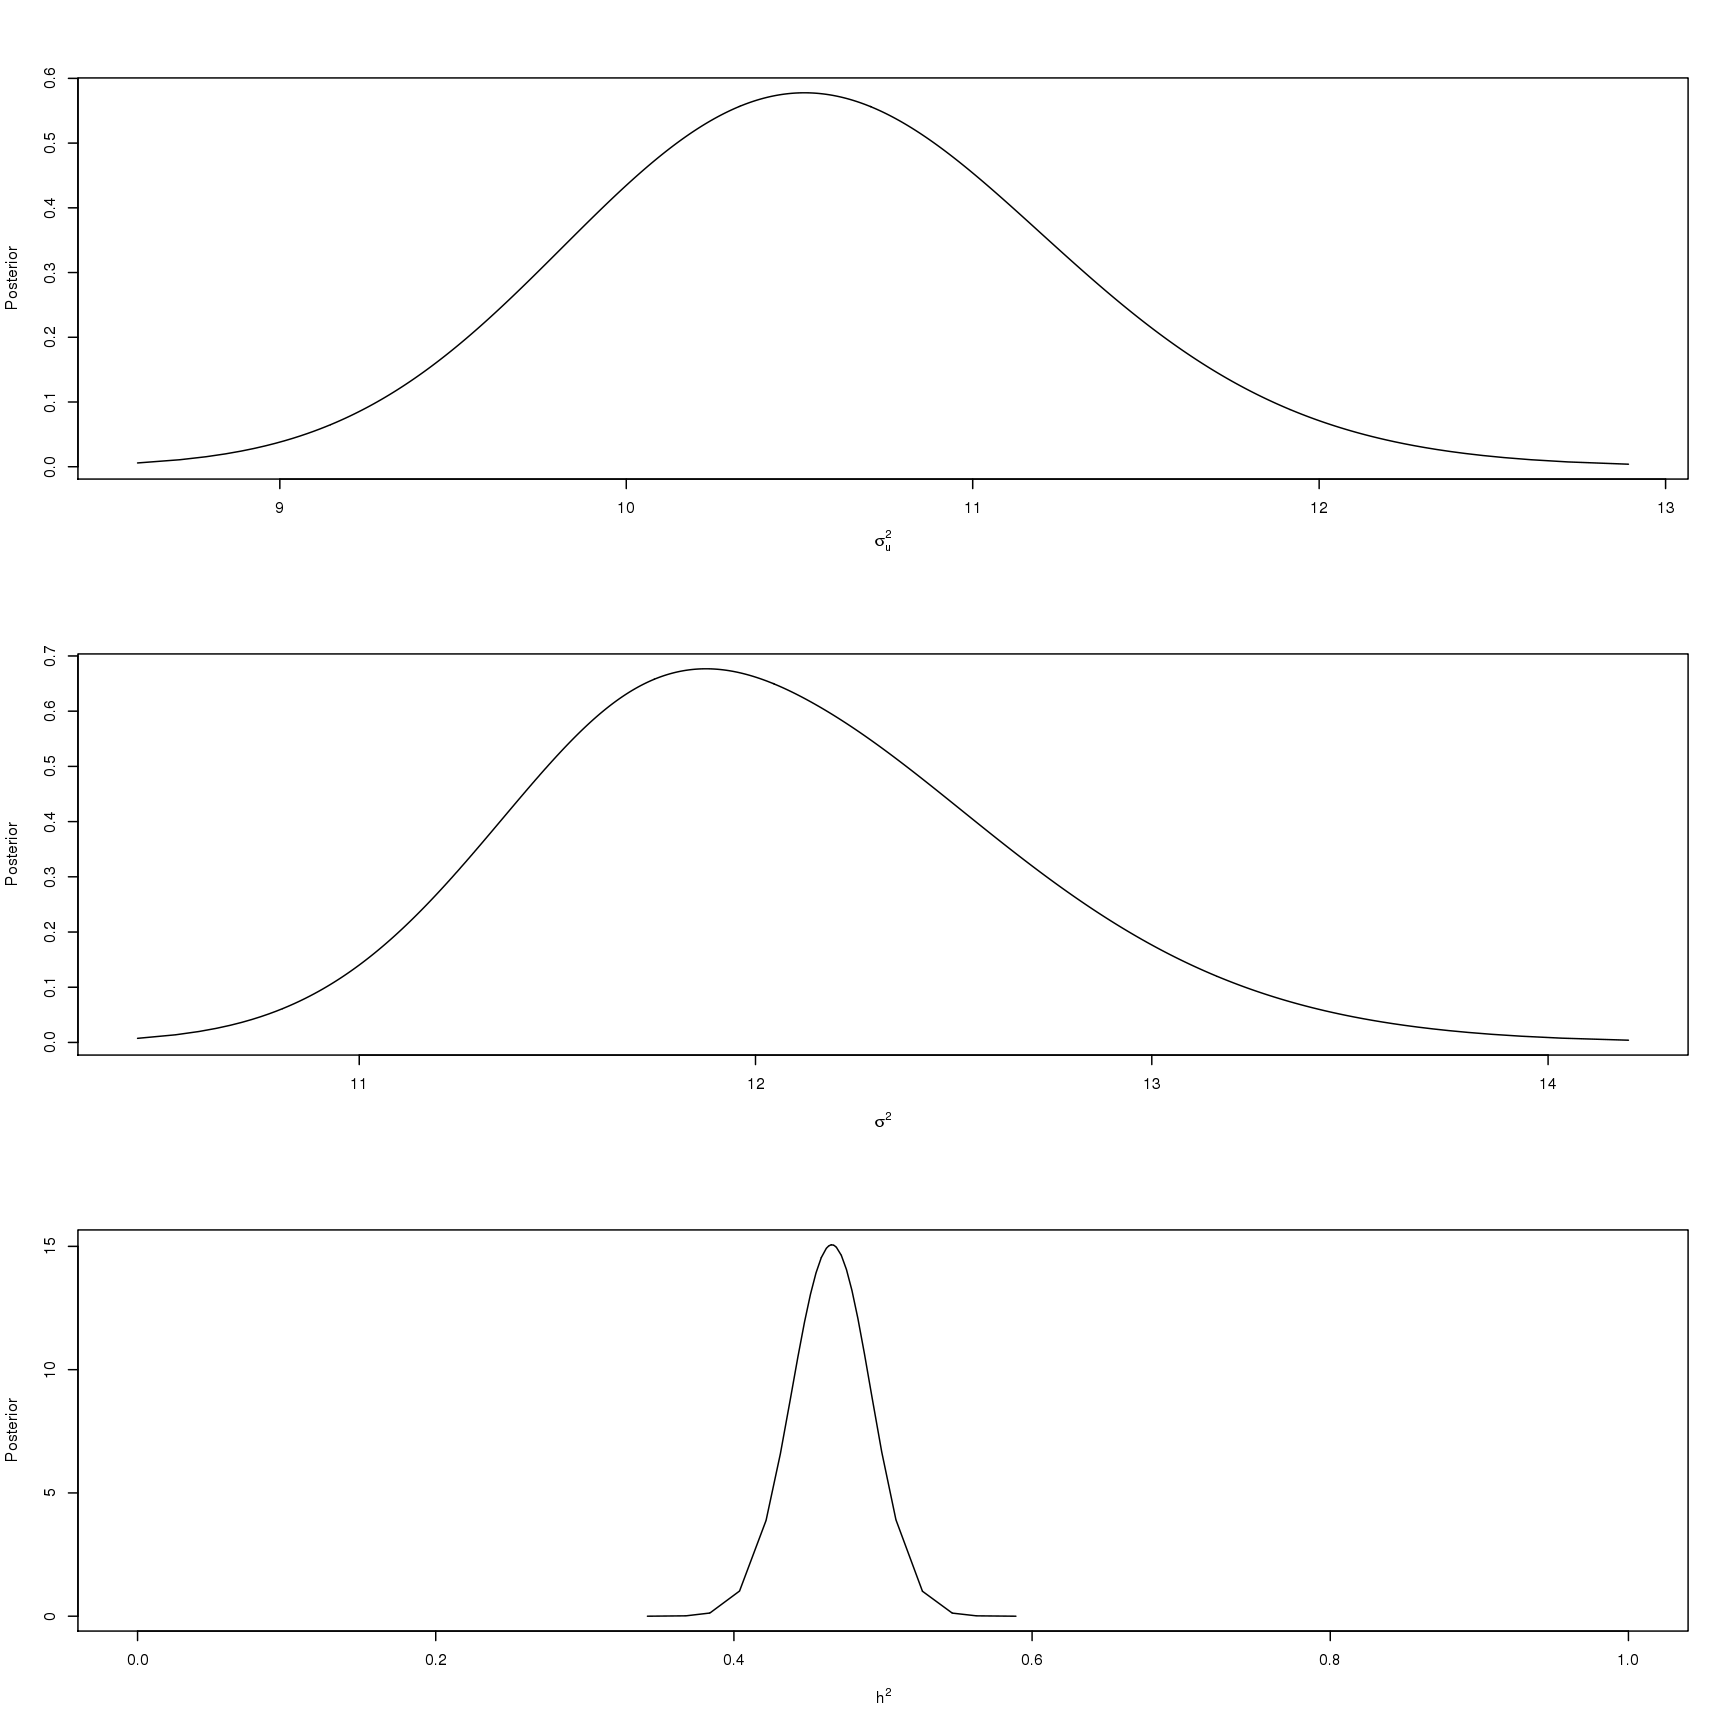
\includegraphics[width=0.8\textwidth, trim = 0 20 0 20, clip]{h2-017}
\caption{Posterior distributions according to package \pkg{AnimalINLA}.}
\label{fgh:animalinla}
\end{figure}

% \subsubsection{Using GRM}
By inspecting the structure of object \texttt{xx} above, we could build 
an compatible object to one from \verb/compute.Ainverse/ function 
% as follows,
% %
% \begin{CodeChunk}
% \begin{CodeInput}
% R> g <- ReadGRM("GRM")
% R> gi <- solve(g$GRM)
% R> k2l <- matrix(NA, N * (N + 1) / 2, 3) 
% R> L <- 1
% R> for (i in seq_len(N)) {
% +    for (j in 1:i) {
% +       k2l[L, ] <- c(j, i, gi[i, j])
% +        L <- L + 1
% +    }
% +  }
% R> x <- list()  
% R> x$Ainverse <- k2l[k2l[, 3] != 0, ]
% R> x$map <- cbind(trios[, 2], seq_len(N))
% R> class(x) <- "ped"
% R> fit <- animal.inla(response = "r", fixed = NULL, 
% +    genetic = "id", Ainverse = x, type.data = "gaussian", data = p2, 
% +    sigma.e = TRUE, dic = TRUE)
% \end{CodeInput}
% \end{CodeChunk}
% %
% where function \verb/ReadGRMBin/ reads in the files
% \texttt{GRM.grm.gz}, \texttt{GRM.grm.id} as
% generated from package \pkg{GCTA} in Section~\ref{fgh:freq} into
% object \texttt{g}, which is in turn inversed and transferred into a
% long-format matrix called \texttt{k2l} and fed into
% \verb/animal.inla/. 
but the GRM looses the sparseness in the kinship matrix from family
structure so is expected to be slower compared to GCTA.

\subsubsection[BLR]{\pkg{BLR}}
Our call is as follows,
%
\begin{CodeChunk}
\begin{CodeInput}
R> y <- as.matrix(r)
R> eps <- 0.1
R> m <- BLR(y, 
+    GF = list(ID = seq_len(N), A = g$GRM + diag(eps, N)),
+    prior = list(varU = list(df = 3, S = 4), varE = list(df = 3, S = 4)),
+    nIter = 500000, burnIn = 150000, thin = 1, saveAt = "fgh.BLR_")
R> attach(m)
R> varU
\end{CodeInput}
\begin{CodeOutput}
         [,1]
[1,] 10.37756
\end{CodeOutput}
\begin{CodeInput}
R> varE
\end{CodeInput}
\begin{CodeOutput}
        [,1]
[1] 11.29452
\end{CodeOutput}
\begin{CodeInput}
R> varU / ((1 + eps) * varU + varE)
\end{CodeInput}
\begin{CodeOutput}
          [,1]
[1,] 0.4569633
\end{CodeOutput}
\begin{CodeInput}
R> detach(m)
R> U <- as.mcmc(scan("fgh.BLR_varU.dat")[-(1:150000)])
R> E <- as.mcmc(scan("fgh.BLR_varE.dat")[-(1:150000)])
R> e <- as.mcmc(cbind(U, E, h2 = U / ((1 + eps) * U + E)))
R> summary(e)$statistics
\end{CodeInput}
\begin{CodeOutput}
         Mean         SD     Naive SE Time-series SE
U  10.3755704 0.63883841 6.929175e-04    0.004220765
E  11.2960400 0.55007729 5.966426e-04    0.003455728
h2  0.4567216 0.02375862 2.576984e-05    0.000160990
\end{CodeOutput}
\begin{CodeInput}
R> HPDinterval(e)
\end{CodeInput}
\begin{CodeOutput}
        lower      upper
U   9.1322010 11.6339900
E  10.2325900 12.3829900
h2  0.4103476  0.5032604
attr(,"Probability")
[1] 0.95
\end{CodeOutput}
\end{CodeChunk}
%
the columns and rows of the GRM are indexed in the object
\texttt{g\$id} whose ordering was used to compromise with that of the
phenotypic data.  The argument \texttt{bF} specifies flat priors for
regression coefficients earlier. The argument \texttt{A} is a
``symmetric, positive definite'' matrix \citep{deloscampos13}. The
priors for the polygenic (\texttt{varU}) and residual (\texttt{varE})
variances follow \cite{deloscampos13} as scaled inverse
$\chi^2$ with expectation $S/(\mathit{df}-2),
S=\VAR(y)(1-h^2)(\mathit{df}-2)$. This is roughly the same for both
variances. The perturbation
$\epsilon=0.1$ has enabled the GRM to be positive definite. Note that
the \verb/saveAt/ option informs the function to keep values of
\texttt{bF}, \texttt{varU} and \texttt{varE} at each iteration to
\texttt{fgh.BLR\_bF.dat}, \texttt{fgh.BLR\_varU.dat} and
\texttt{fgh.BLR\_varE.dat}, respectively. Figure~\ref{fgh:blr} shows the
results of a very long chain (150,000 burn-ins, 350,000 iterations).
The sequences were also converted into an `\code{mcmc}' object used
  in package \pkg{coda} from which we obtained the HPD interval via
  function \verb/HPDinterval/.  The density plot is indeed similar to
  Figure~\ref{fgh:animalinla}.
%
\begin{CodeChunk}
\begin{CodeInput}
R> plot(e)
\end{CodeInput}
\end{CodeChunk}
%
\begin{figure}[t!]
\centering
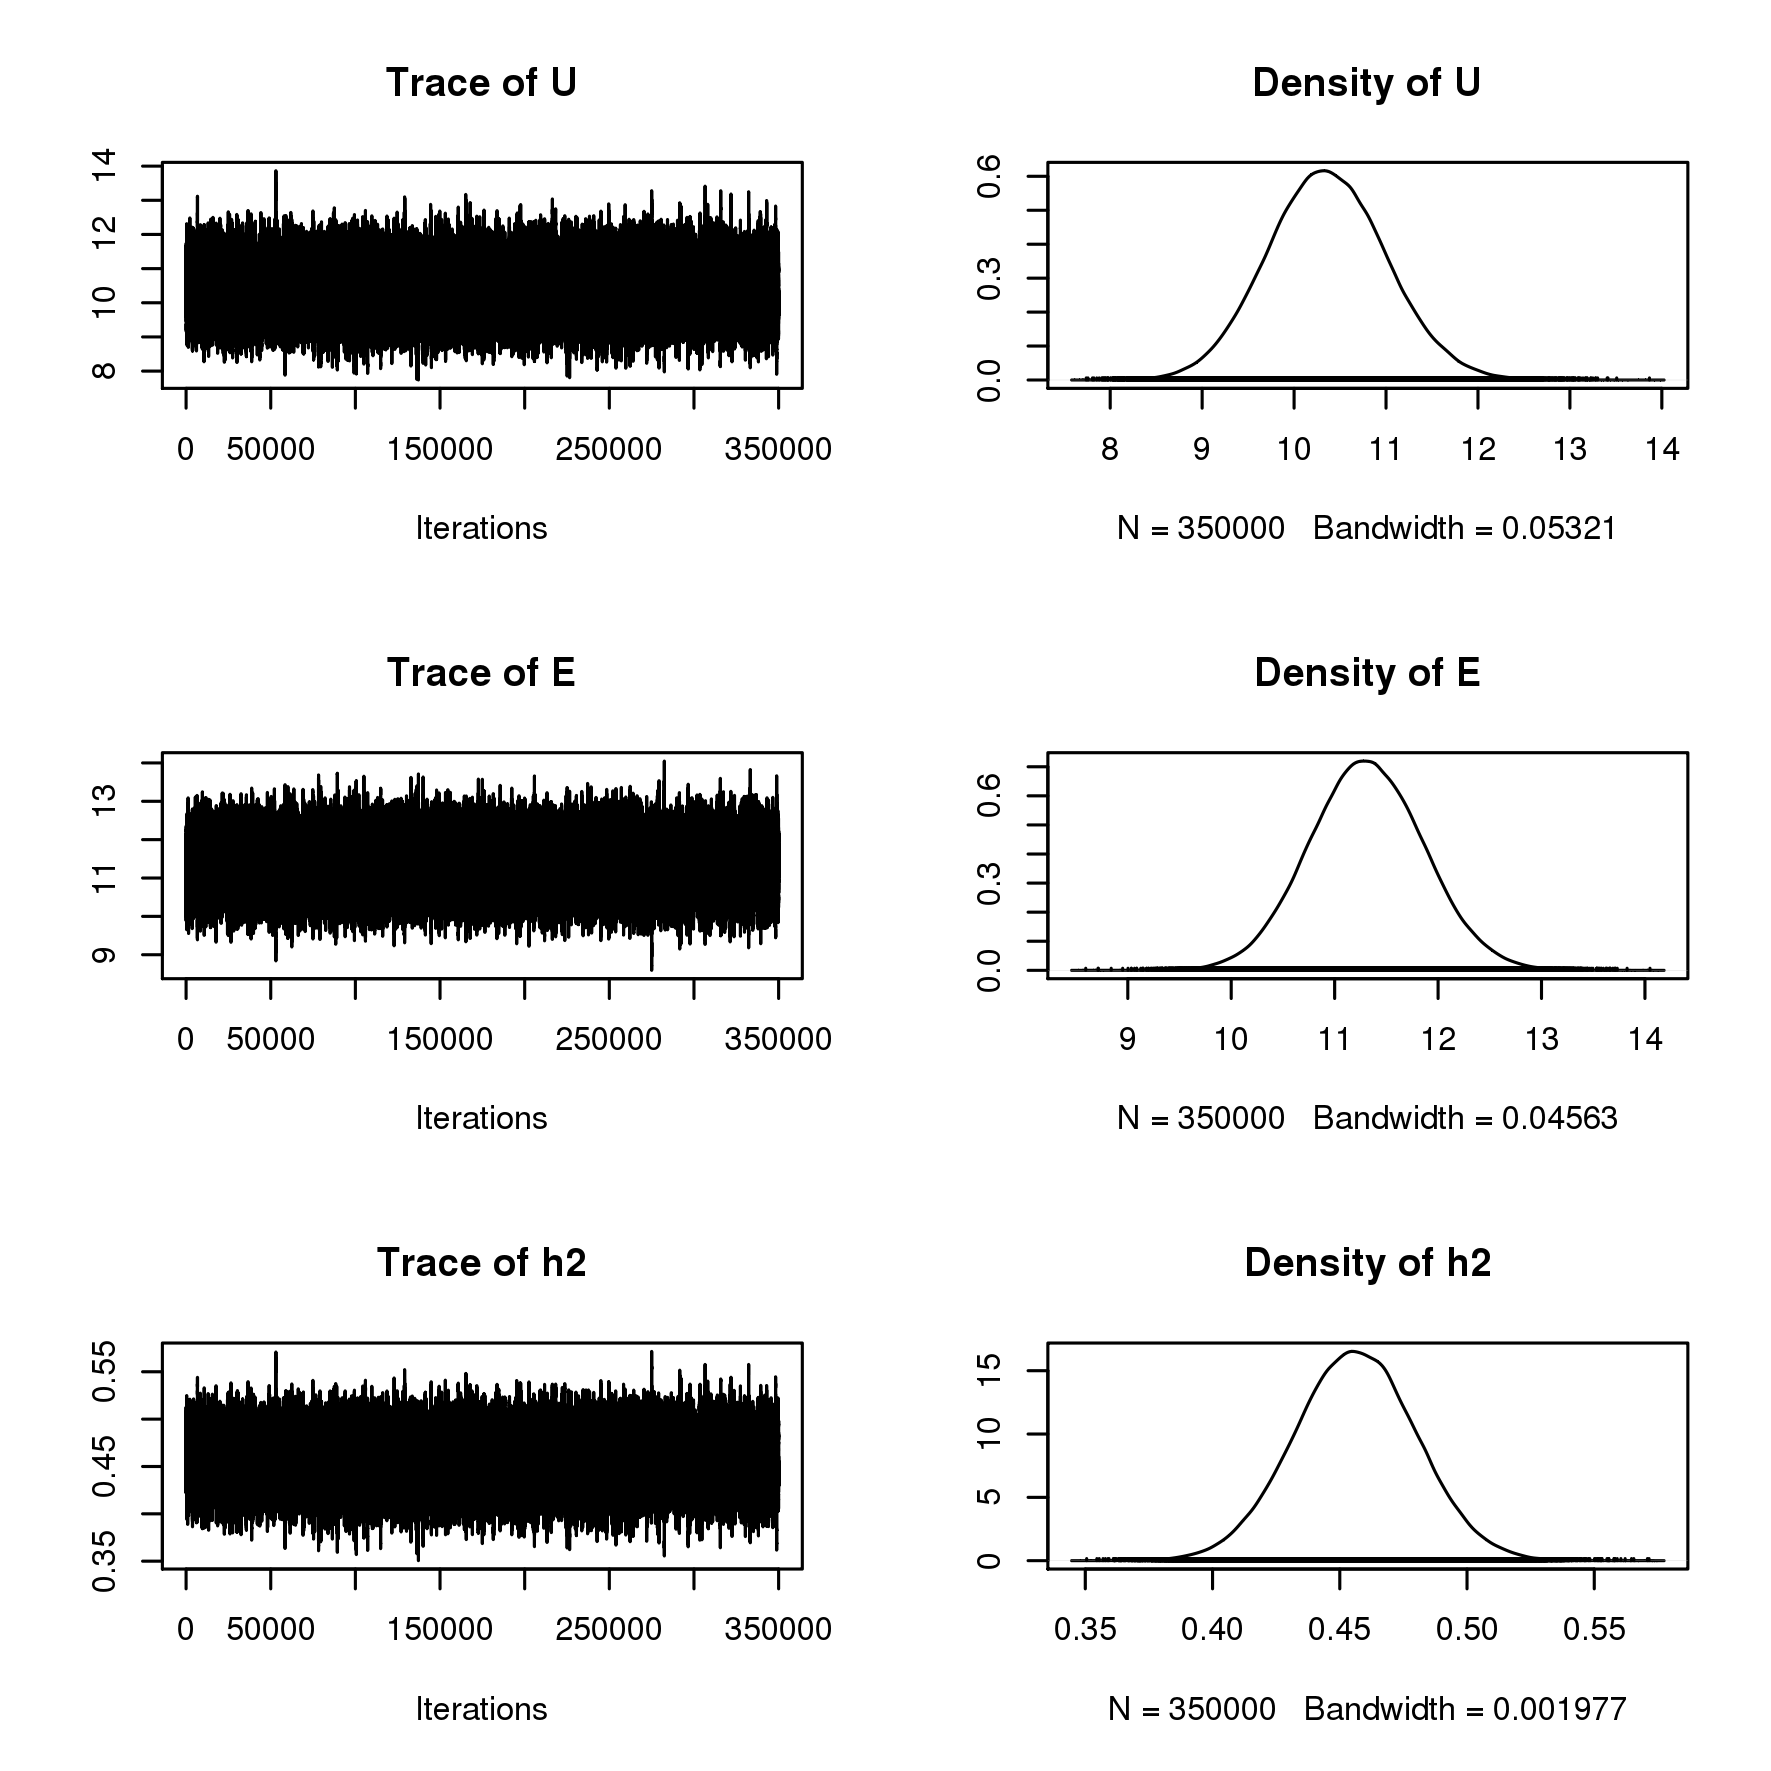
\includegraphics[width=\textwidth, trim = 0 10 0 10, clip]{fgh_BLR.png}
\caption{Posterior distributions of polygenic variance (top), 
residual variance (middle) and $h^2$ (bottom) according to package \pkg{BLR}.}
\label{fgh:blr}
\end{figure}

\section{Summary}

We implemented Bayesian linear mixed models that involve a direct use
of the relationship matrix. Generic software such as \pkg{JAGS} or
\proglang{Stan} renders greater simplicity than purpose-written
software and more flexibility for complex models. Through data
analysis we showed that the frequentist and Bayesian approaches can
give comparable point estimates but the latter is desirable with its
ability to use prior information and produce posterior
distributions. For large samples, unlike the usual availability of
family structures and therefore fast on-the-fly calculation of the
inverse of the precision matrix involving polygenic variance
\citep{waldmann09, damgaard07} they have great difficulty in dealing
with large genomic matrices. We therefore exploited matrix
decomposition and parallel computation. We also compiled \pkg{JAGS}
using both \pkg{LAPACK} and \pkg{Intel MKL}. Given that the computing
time remains prohibitive, we further used approximate Bayesian
inference such as Laplace approximation, in particular \pkg{INLA} as
in package \pkg{AnimalINLA}, which was again humbled by the high
dimensionality and non-sparsity density of the GRM. Our analysis also
naturally called up a number of packages in the \proglang{R} system
with its ability for data management, powerful programming and
modeling.

The implementation has not been seen in the literature and
\proglang{Stan} gave comparable results to the usual REML estimation
and those obtained with package \pkg{JAGS}. Our setup enables relationship
matrix from either family or population data directly into a polygenic
model. The comparison of both types of relationship matrices is now
possible with package \pkg{MCMCglmm} from which a function \verb/MCMCgrm/ was
implemented in package \pkg{gap}. Package \pkg{BLR} runs faster but would fail with a
non-positive definite $G$ matrix. Unlike \cite{guo91}, our approach
does not involve repeated inversion or factorization of the
variance-covariance matrix at the sampling stage and has enabled
analysis package \pkg{BLR}. The analysis also went
beyond our previous experiment \citep{zhao12}, whose focus was only on
frequentist approaches. A reviewer pointed out work by \cite{bae14}
noting previous work on decomposition and conditioning by
\citet{waldman08, hallander10} where they ``proposed an approach based
on a decomposition of the multivariate Normal distribution of the
random effects into univariate Normal distributions using conditional
distributions'' but ``fails to produce accurate results with large
multigenerational families'' though the authors ``were not able to
pinpoint the reason for the apparent discrepancy'' (between the
conditioning and singular value decomposition). In essence, the model
as in \cite{bae14} has a covariance structure
\begin{equation}
V = 2\sigma_g^2\left( \begin{array}{cccc}
K_1 & \hfill & \hfill & \hfill \\
\hfill & K_2 & \hfill & \hfill \\
\hfill & \hfill & \ddots \hfill \\
\hfill & \hfill & \hfill & K_m \\
\end{array} \right)+\sigma^2I,
\end{equation}
where $K_i$ are the kinship matrices associate with a particular family $i$,
$i=1, \ldots, m$. In our case, the GRM does not have the block structure. In
\cite{hallander10}, dominance effects were also modeled and in principle
can be included in our approach similar to GRM.

We hope that our work will facilitate exploration of other practical issues
of Bayesian linear mixed models with polygenic effects, some of which are
highlighted here. 

\subsection{Non-genetic effects}
Although we have focused on the polygenic effects, their non-genetic 
counterparts can be an indispensable part of the research. For instance, BMI may
be linked to lifestyle and psychosocial factors such as diet, physical 
activity and mental health. SNP effects are now commonly derived as part
of a GWAS from the so-called mixed linear effects model involving polygenic
effects and SNP dosage as fixed effects. Gene-environment interactions
are also important. 

For non-genetic effects, the $g$-prior \citep{zellner86} is often used. In our
notation, this amounts to $\beta\sim \mathit{MVN}(\beta_0, a\sigma^2(X^\top X)^{-1})$ 
where $\beta_0$ is a hyperparameter and $a$ a positive scalar often chosen 
to be the sample size, noting the use of $a$ instead of $g$ as in the 
literature is simply to avoid confusion with the polygenic effects $g$
throughout this paper and elsewhere. The prior can facilitate model comparison
since in the case of multiple linear regression closed form regression
coefficients can be obtained but some undesirable property in model 
comparison has also been documented \citep[e.g.,][]{pericchi05}.

\subsection{Efficient implementation}
The polygenic modeling would benefit greatly from a truly efficient
Bayesian computation software system involving fine-tuned algorithms.
Our limited experience showed that \pkg{JAGS} and \proglang{Stan}
are feasible for moderate sample size ($N\approx 1,000$) but become very 
time-consuming when it gets larger. Besides approaches described in Section~\ref{pc}, 
\pkg{JAGS} can be compiled to use multicore facility. Recent versions of
\pkg{rstan} actually have an option \verb/cores/ to automatically use all
available cores. We do not attempt to elaborate this here as it is an 
active and evolving area with work such as \cite{kruschke15} giving 
further information. 

Our work suggests that a combination of generic Bayesian analysis
systems such as \pkg{JAGS} and \proglang{Stan} together with specific
software such as package \pkg{BLR} will still be appealing. For the
Framingham data, we also experimented with package \pkg{MCMCglmm} and
the function \verb/MCMCgrm/; both took considerably longer than
package \pkg{BLR}. \cite{ahlinder13} made a further attempt to speed
up calculations by treating $\beta$ and $u$ as nuisance parameters in
the posterior distribution
$$\Prob(\beta,u,\sigma_\beta^2,\sigma_g^2,\sigma^2|y) 
\propto 
\Prob(y|\beta,u,\sigma^2)\Prob(\beta|\sigma_\beta^2)\Prob(u|\sigma_u^2)\Prob(\sigma_\beta^2)\Prob(\sigma_u^2)\Prob(\sigma^2)$$
 so that $\Prob(\sigma_\beta^2,\sigma_u^2,\sigma^2|y)\propto$ 
$\Prob(\sigma_\beta^2)\Prob(\sigma_u^2)\Prob(\sigma^2)$ $\int 
\Prob(y|\beta,u,\sigma^2)\Prob(\beta|\sigma_\beta^2)\Prob(u|\sigma_u^2)d\beta 
du$ but 
the likelihood specification is still involved. Bayesian inference using 
Laplace approximation in the spirit of \pkg{INLA} is also available from 
\pkg{LaplacesDemon} \citep{LaplacesDemon} and a counterpart 
\pkg{LaplacesDemonCpp} \citep{LaplacesDemonCpp} with an incremental 
inclusion of \proglang{C++}.

\subsection{Missing outcome}
It is more involved to allow for missing data. We did not address this explicitly
and in general that is possible \citep[p.~176]{stan}. However, we took advantage
of the built-in mechanism in package \pkg{BLR}. For the Meyer data without filling the
missing data, the results are obtained as follows,
%
\begin{Schunk}
\begin{Sinput}
R> set.seed(1234567)
R> meyer <- within(meyer, {
+    yNa <- y
+    g1 <- ifelse(generation == 1, 1, 0)
+    g2 <- ifelse(generation == 2, 1, 0)
+    id <- animal
+    animal <- ifelse(!is.na(animal), animal, 0)
+    dam <- ifelse(!is.na(dam), dam, 0)
+    sire <- ifelse(!is.na(sire), sire, 0)
+  })
R> G <- kin.morgan(meyer)$kin.matrix * 2
R> library("regress")
R> r <- regress(y ~ -1 + g1 + g2, ~ G, data = meyer)
R> r
R> library("BLR")
R> attach(meyer)
R> X <- as.matrix(meyer[c("g1", "g2")])
R> m <- BLR(yNa, XF = X, GF = list(ID = 1:nrow(G), A = G),
+    prior = list(varE = list(df = 1, S = 0.25), 
+    varU = list(df = 1, S = 0.63)),
+    nIter = 5000, burnIn = 500, thin = 1, saveAt = "meyer.BLR")
R> with(r, h2G(sigma, sigma.cov))
\end{Sinput}
\begin{Soutput}
Vp = 104.091 SE = 9.925092 
h2G = 0.3042677 SE = 0.1147779 
\end{Soutput}
\begin{Sinput}
R> names(m)
\end{Sinput}
\begin{Soutput}
 [1] "y"       "weights" "mu"      "varE"    "yHat"    "SD.yHat"
 [7] "whichNa" "fit"     "bF"      "SD.bF"   "u"       "SD.u"   
[13] "varU"    "prior"   "nIter"   "burnIn"  "thin"   
\end{Soutput}
\begin{Sinput}
R> attach(m)
R> yHat[whichNa]
\end{Sinput}
\begin{Soutput}
numeric(0)
\end{Soutput}
\begin{Sinput}
R> mu
\end{Sinput}
\begin{Soutput}
[1] 327.9259
\end{Soutput}
\begin{Sinput}
R> bF
\end{Sinput}
\begin{Soutput}
        g1         g2 
-105.11362  -89.52557 
\end{Soutput}
\begin{Sinput}
R> mu + bF
\end{Sinput}
\begin{Soutput}
      g1       g2 
222.8123 238.4004 
\end{Soutput}
\begin{Sinput}
R> varU
\end{Sinput}
\begin{Soutput}
         [,1]
[1,] 29.66097
\end{Soutput}
\begin{Sinput}
R> varE
\end{Sinput}
\begin{Soutput}
[1] 74.08534
\end{Soutput}
\begin{Sinput}
R> varU / (varU + varE)
\end{Sinput}
\begin{Soutput}
         [,1]
[1,] 0.285899
\end{Soutput}
\end{Schunk}
%
with which we would be more comfortable. It seems that both frequentist
and Bayesian approaches yielded smaller variance components compared to
the imputation of missing outcome a priori. From the quantity \texttt{mu}
and \texttt{bF} we are able to recover regression coefficients for the
fixed effects comparable to what we have seen earlier. Furthermore, a
vector \texttt{whichNa} indicates which observation has a missing outcome
so that \texttt{yHat[whichNa]} contains predicted values for those missing
outcomes.

Package \pkg{GCTA} can give heritability and standard error estimates
for a quantitative trait based on a large number of SNPs. The
documentation data involves a quantitative trait for 3,925 individuals
and 1,000 SNPs, leading to $h^2 (\mathit{SE})=0.022$ $(0.009)$. 
% We conducted a bootstrap experiment where we got an
% estimate of 0.191 (0.023), suggesting that some improvement can be
% made with respect to the usual likelihood estimate. 
Now we ran 5,000 burn-ins and 10,000 iterations with package \pkg{BLR} 
and obtained 0.119 (0.001) and 95\% HPD interval (0.098--0.142), still 
slightly higher than that based on REML estimation.

Gaussian outcome is but one of many scenarios for which polygenic effects 
can be included. Our frequentist counterparts include packages \pkg{regress},
\pkg{pedigreemm} \citep{vazquez10} and \pkg{coxme} \citep{coxme}, all 
in the \proglang{R} environment. They could involve problems with outcomes 
being binary, Poisson, time-to-event, etc. Our focus was on $h^2$ and 
there should be some similarity when we approach other indicators from the 
mixed models such as coefficient of determination ($R^2$) 
\citep{nakagawa13}.

\section*{Acknowledgments}

The work derived from participation of the Genetic Analysis Workshops
(GAW) involving porting the \proglang{S-PLUS} package
\pkg{kinship}, developed at the Mayo Clinic, to \proglang{R} 
\citep{zhao05}. We wish to thank Prof.~Terry Therneau and colleagues for 
many advices throughout the eight-year maintenance of the \proglang{R} package \pkg{kinship}, 
whose functions are now contained in packages \pkg{bdsmatrix} 
\citep{bdsmatrix}, \pkg{coxme} and \pkg{kinship2} all available from 
CRAN. Two anonymous reviewers, associate editor Prof.~Donald Hedeker 
from University of Chicago and the Editors have made numerous suggestions and recommendations 
leading to a much improved presentation.

\newpage
\bibliography{ref}

\end{document}
